%% fig_weilcube.tex   (generated by make_core.py; do not edit by hand)
%% The 4-cube of monomials w(T), with the bipartition by the parity of |T| that separates the two generators of the Weil line.
\documentclass[tikz,border=8pt]{standalone}
\usepackage{amsmath,amssymb}
\usetikzlibrary{arrows.meta,calc}
%% palette.tex -- shared colour definitions for the figures
\definecolor{PInk}{RGB}{26,32,44}
\definecolor{PBlue}{RGB}{37,82,139}
\definecolor{PTeal}{RGB}{23,127,125}
\definecolor{POchre}{RGB}{193,138,44}
\definecolor{PClay}{RGB}{178,74,58}
\definecolor{PSlate}{RGB}{108,122,137}
\definecolor{PViolet}{RGB}{110,86,150}
\definecolor{WBlue}{RGB}{223,234,246}
\definecolor{WTeal}{RGB}{220,238,236}
\definecolor{WOchre}{RGB}{250,240,218}
\definecolor{WClay}{RGB}{247,229,224}
\definecolor{WSlate}{RGB}{238,241,244}
\definecolor{PMag}{RGB}{158,58,110}
\definecolor{PGrass}{RGB}{62,124,66}
\definecolor{PAmber}{RGB}{214,112,38}
\definecolor{PIndigo}{RGB}{58,64,140}
\definecolor{PRule}{RGB}{176,186,197}

%% shared macros so the standalone figures match the paper
\providecommand{\QQ}{\mathbb{Q}}
\providecommand{\ZZ}{\mathbb{Z}}
\providecommand{\RR}{\mathbb{R}}
\providecommand{\CC}{\mathbb{C}}
\providecommand{\PP}{\mathbb{P}}
\providecommand{\Kx}{K^{\times}}
\providecommand{\HW}{W}
\providecommand{\Nm}{\mathrm{N}}
\providecommand{\Hdg}{\mathrm{Hdg}}
\providecommand{\NS}{\mathrm{NS}}
\providecommand{\cA}{\mathcal{A}}
\providecommand{\cD}{\mathcal{D}}
\providecommand{\cF}{\mathcal{F}}
\providecommand{\cP}{\mathcal{P}}
\providecommand{\cO}{\mathcal{O}}
\providecommand{\cQ}{\mathcal{Q}}
\providecommand{\bbar}[1]{\overline{#1}}
\providecommand{\ch}{\operatorname{ch}}
\providecommand{\End}{\mathrm{End}}

\begin{document}
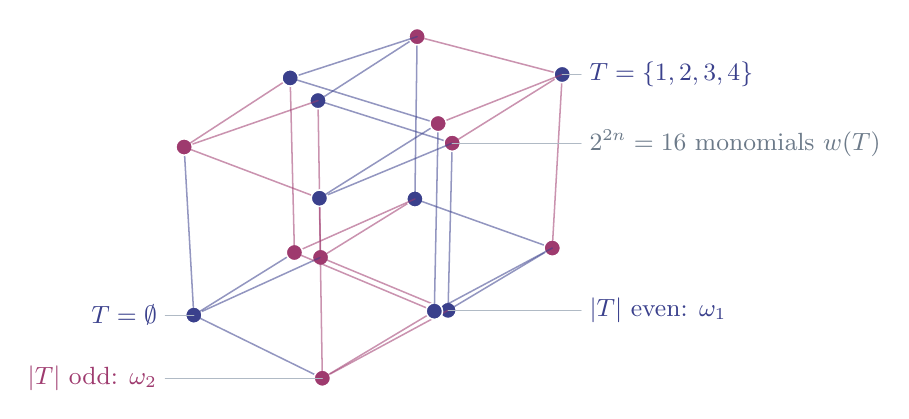
\begin{tikzpicture}[x=1cm,y=1cm,line join=round,line cap=round,
  font=\small,text=PInk]
  \node[circle,fill=PMag,draw=white,line width=0.55pt,inner sep=2.1pt] at (-0.6449,-0.7389) {};
  \draw[PMag,line width=0.55pt,opacity=0.55] (-0.6449,-0.7389) -- (0.5536,0.0029);
  \node[circle,fill=PIndigo,draw=white,line width=0.55pt,inner sep=2.1pt] at (0.5536,0.0029) {};
  \draw[PMag,line width=0.55pt,opacity=0.55] (-0.6449,-0.7389) -- (-0.6771,1.2523);
  \draw[PMag,line width=0.55pt,opacity=0.55] (-0.6449,-0.7389) -- (0.9745,-1.4117);
  \draw[PIndigo,line width=0.55pt,opacity=0.55] (0.5536,0.0029) -- (0.5816,2.0642);
  \draw[PIndigo,line width=0.55pt,opacity=0.55] (-2.2545,-1.4726) -- (-0.6449,-0.7389);
  \node[circle,fill=PIndigo,draw=white,line width=0.55pt,inner sep=2.1pt] at (-0.6771,1.2523) {};
  \draw[PIndigo,line width=0.55pt,opacity=0.55] (0.5536,0.0029) -- (2.2981,-0.6206);
  \draw[PIndigo,line width=0.55pt,opacity=0.55] (-0.6771,1.2523) -- (0.5816,2.0642);
  \draw[PMag,line width=0.55pt,opacity=0.55] (-0.9765,-0.6771) -- (0.5536,0.0029);
  \node[circle,fill=PMag,draw=white,line width=0.55pt,inner sep=2.1pt] at (0.5816,2.0642) {};
  \node[circle,fill=PIndigo,draw=white,line width=0.55pt,inner sep=2.1pt] at (0.9745,-1.4117) {};
  \node[circle,fill=PIndigo,draw=white,line width=0.55pt,inner sep=2.1pt] at (-2.2545,-1.4726) {};
  \draw[PIndigo,line width=0.55pt,opacity=0.55] (0.9745,-1.4117) -- (2.2981,-0.6206);
  \draw[PIndigo,line width=0.55pt,opacity=0.55] (-0.6771,1.2523) -- (1.0272,0.7117);
  \draw[PMag,line width=0.55pt,opacity=0.55] (-2.3772,0.6625) -- (-0.6771,1.2523);
  \draw[PIndigo,line width=0.55pt,opacity=0.55] (-2.2545,-1.4726) -- (-0.9765,-0.6771);
  \node[circle,fill=PMag,draw=white,line width=0.55pt,inner sep=2.1pt] at (2.2981,-0.6206) {};
  \node[circle,fill=PMag,draw=white,line width=0.55pt,inner sep=2.1pt] at (-0.9765,-0.6771) {};
  \draw[PIndigo,line width=0.55pt,opacity=0.55] (0.9745,-1.4117) -- (1.0272,0.7117);
  \draw[PMag,line width=0.55pt,opacity=0.55] (0.5816,2.0642) -- (2.4245,1.5840);
  \draw[PIndigo,line width=0.55pt,opacity=0.55] (-1.0306,1.5402) -- (0.5816,2.0642);
  \draw[PIndigo,line width=0.55pt,opacity=0.55] (-2.2545,-1.4726) -- (-2.3772,0.6625);
  \draw[PMag,line width=0.55pt,opacity=0.55] (2.2981,-0.6206) -- (2.4245,1.5840);
  \draw[PMag,line width=0.55pt,opacity=0.55] (-0.6223,-2.2740) -- (0.9745,-1.4117);
  \draw[PIndigo,line width=0.55pt,opacity=0.55] (-2.2545,-1.4726) -- (-0.6223,-2.2740);
  \draw[PMag,line width=0.55pt,opacity=0.55] (-0.9765,-0.6771) -- (-1.0306,1.5402);
  \node[circle,fill=PMag,draw=white,line width=0.55pt,inner sep=2.1pt] at (1.0272,0.7117) {};
  \node[circle,fill=PMag,draw=white,line width=0.55pt,inner sep=2.1pt] at (-2.3772,0.6625) {};
  \draw[PMag,line width=0.55pt,opacity=0.55] (1.0272,0.7117) -- (2.4245,1.5840);
  \draw[PIndigo,line width=0.55pt,opacity=0.55] (0.8003,-1.4220) -- (2.2981,-0.6206);
  \draw[PMag,line width=0.55pt,opacity=0.55] (-0.9765,-0.6771) -- (0.8003,-1.4220);
  \draw[PMag,line width=0.55pt,opacity=0.55] (-2.3772,0.6625) -- (-1.0306,1.5402);
  \node[circle,fill=PIndigo,draw=white,line width=0.55pt,inner sep=2.1pt] at (2.4245,1.5840) {};
  \node[circle,fill=PIndigo,draw=white,line width=0.55pt,inner sep=2.1pt] at (-1.0306,1.5402) {};
  \node[circle,fill=PMag,draw=white,line width=0.55pt,inner sep=2.1pt] at (-0.6223,-2.2740) {};
  \draw[PIndigo,line width=0.55pt,opacity=0.55] (-0.6593,0.0124) -- (1.0272,0.7117);
  \draw[PMag,line width=0.55pt,opacity=0.55] (-0.6223,-2.2740) -- (0.8003,-1.4220);
  \draw[PMag,line width=0.55pt,opacity=0.55] (-2.3772,0.6625) -- (-0.6593,0.0124);
  \node[circle,fill=PIndigo,draw=white,line width=0.55pt,inner sep=2.1pt] at (0.8003,-1.4220) {};
  \draw[PMag,line width=0.55pt,opacity=0.55] (0.8488,0.9608) -- (2.4245,1.5840);
  \draw[PMag,line width=0.55pt,opacity=0.55] (-0.6223,-2.2740) -- (-0.6593,0.0124);
  \draw[PIndigo,line width=0.55pt,opacity=0.55] (-1.0306,1.5402) -- (0.8488,0.9608);
  \draw[PIndigo,line width=0.55pt,opacity=0.55] (0.8003,-1.4220) -- (0.8488,0.9608);
  \node[circle,fill=PIndigo,draw=white,line width=0.55pt,inner sep=2.1pt] at (-0.6593,0.0124) {};
  \draw[PIndigo,line width=0.55pt,opacity=0.55] (-0.6593,0.0124) -- (0.8488,0.9608);
  \node[circle,fill=PMag,draw=white,line width=0.55pt,inner sep=2.1pt] at (0.8488,0.9608) {};
  \draw[PRule,line width=0.35pt] (-2.6172,-1.4726) -- (-2.2545,-1.4726);
  \node[text=PIndigo,anchor=east,inner sep=0pt] at (-2.7172,-1.4726) {$T=\emptyset$};
  \draw[PRule,line width=0.35pt] (-2.6172,-2.2740) -- (-0.6223,-2.2740);
  \node[text=PMag,anchor=east,inner sep=0pt] at (-2.7172,-2.2740) {$|T|$ odd: $\omega_{2}$};
  \draw[PRule,line width=0.35pt] (2.6645,1.5840) -- (2.4245,1.5840);
  \node[text=PIndigo,anchor=west,inner sep=0pt] at (2.7645,1.5840) {$T=\{1,2,3,4\}$};
  \draw[PRule,line width=0.35pt] (2.6645,0.7117) -- (1.0272,0.7117);
  \node[text=PSlate,anchor=west,inner sep=0pt] at (2.7645,0.7117) {$2^{2n}=16$ monomials $w(T)$};
  \draw[PRule,line width=0.35pt] (2.6645,-1.4117) -- (0.9745,-1.4117);
  \node[text=PIndigo,anchor=west,inner sep=0pt] at (2.7645,-1.4117) {$|T|$ even: $\omega_{1}$};
\end{tikzpicture}
\end{document}
